% This LaTeX was auto-generated from MATLAB code.
% To make changes, update the MATLAB code and export to LaTeX again.

\documentclass{article}

\usepackage[utf8]{inputenc}
\usepackage[T1]{fontenc}
\usepackage{lmodern}
\usepackage{graphicx}
\usepackage{color}
\usepackage{hyperref}
\usepackage{amsmath}
\usepackage{amsfonts}
\usepackage{epstopdf}
\usepackage[table]{xcolor}
\usepackage{matlab}

\sloppy
\epstopdfsetup{outdir=./}
\graphicspath{ {./Mohit_test_images/} }

\begin{document}

\matlabheading{\textbf{Fit experimental data to obtain the values of Qmobile, Ro, and Tdiffusion}}

\begin{matlabcode}
addpath('C:\Users\mrmehta\Downloads\Archive\Code')
cd('C:\Users\mrmehta\Downloads\Archive\Code')
clear all
name = 'RW15';
close all;

% So first we are given our qmax/Ro/tDiff "observations" from the sys id
% part. Let's load those up.
data = Data.load(name,'step');
load(['Results/' name 'RWEstimatesQMobileRoTDiff.mat']);

QMobile = results.estimates.qMobile;
Ro = results.estimates.Ro;
TDiffusion = results.estimates.tDiffusion;

% Our equation is qmobile(k+1) = qmobile(k) - w_q * |i(k)| * dt
% So we need also to have i(k) values. How do we get those? Do average.
% Compute i(k) values, and dt values
I = [];
Dt = [];
startIndex = 1;
for i=1:length(results.rwIndices.rwEnd)
% 	fprintf('RW discharge %g\n',i);
	% Get index of last step of random walk discharge
	index = results.rwIndices.rwEnd(i);
	% Construct a segment from startIndex to index
	segment = Data.getSegments(data,startIndex:index);
	startIndex = index+1;
	% Now, get average current from that segment
	I(i) = mean(abs(segment.current));
	% Get also the dt for this
	Dt(i) = segment.time(end)-segment.time(1);
end

% Now want to implement our equation, and try different values of w_q to
% see that it makes sense
wq = 1.5e-4;
QMobilePredicted(1) = QMobile(1);
for k=2:length(QMobile)
	QMobilePredicted(k) = QMobilePredicted(k-1) - wq*I(k-1)*Dt(k-1);
end
figure;
K = 1:length(QMobile);
plot(K,QMobile,'b.',K,QMobilePredicted,'r.');
title('QMobile Observed and Predicted')
legend('Observed','Predicted');
\end{matlabcode}
\begin{center}
\includegraphics[width=\maxwidth{56.196688409433015em}]{figure_0.eps}
\end{center}
\begin{matlabcode}

% Do the same for Ro
wR = 4e-9;
RoPredicted(1) = Ro(1);
for k=2:length(Ro)
	RoPredicted(k) = RoPredicted(k-1) + wR*I(k-1)*Dt(k-1);
end
figure;
plot(K,Ro,'b.',K,RoPredicted,'r.');
title('Ro Observed and Predicted')
legend('Observed','Predicted');
\end{matlabcode}
\begin{center}
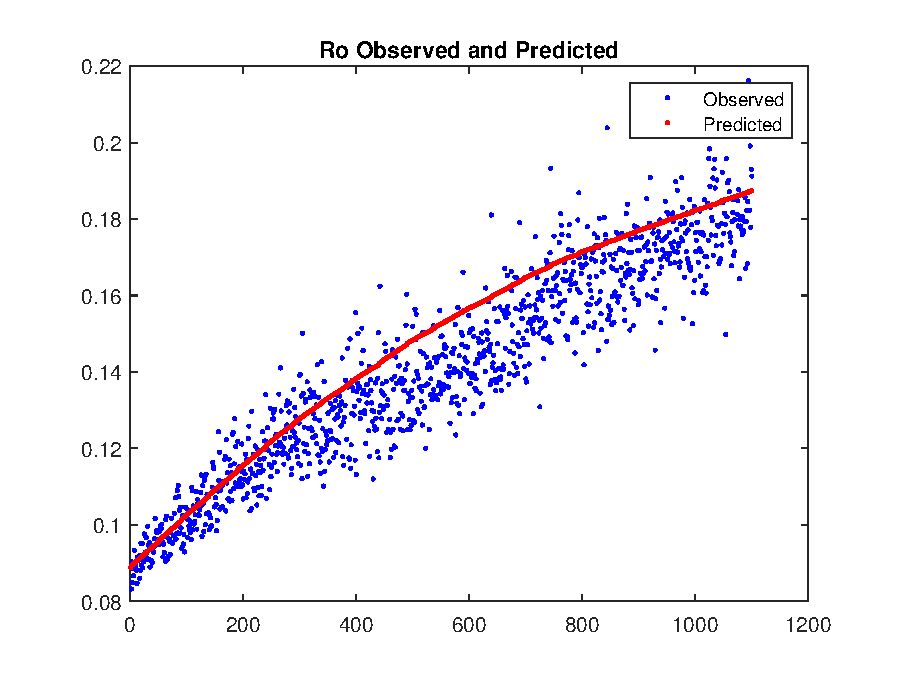
\includegraphics[width=\maxwidth{56.196688409433015em}]{figure_1.eps}
\end{center}
\begin{matlabcode}
% ... and tDiffusion
wTD = 2.2e0;
TDiffusionPredicted(1) = 1e6;
for k=2:length(TDiffusion)
	TDiffusionPredicted(k) = TDiffusionPredicted(k-1) + wTD*I(k-1)*Dt(k-1);
end
figure;
plot(K,TDiffusion.*1e-7,'b.',K,TDiffusionPredicted.*1e-7,'r.');
title('TDiffusion Observed and Predicted')
legend('Observed','Predicted');
\end{matlabcode}
\begin{center}
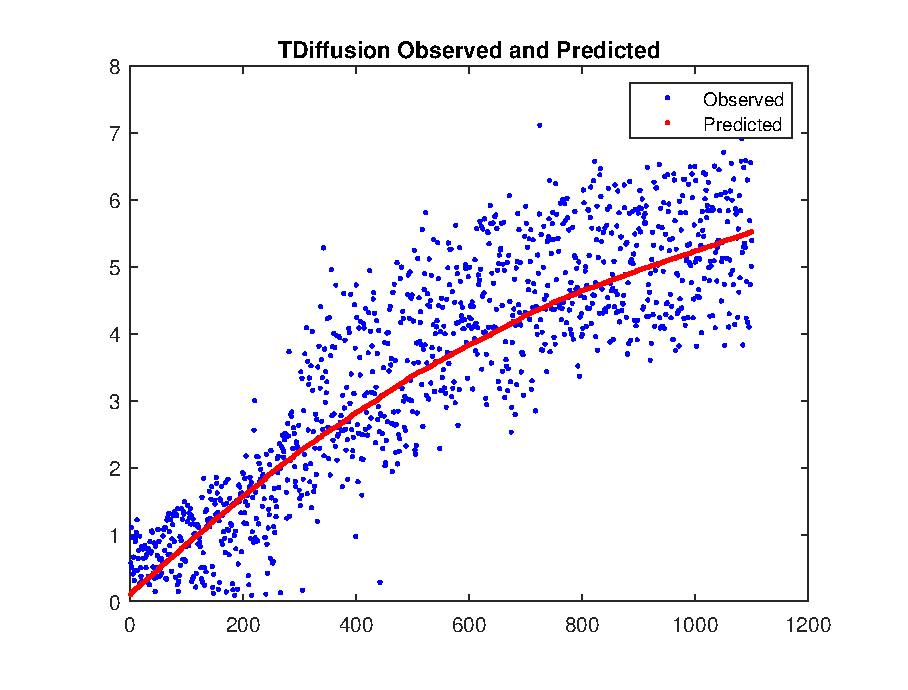
\includegraphics[width=\maxwidth{56.196688409433015em}]{figure_2.eps}
\end{center}


\begin{matlabcode}

% Note that in these plots, plotting against K not t (sample times between
% k values is not constant).

% So that shows that this model seems to be quite good! Now, the question
% is how to estimate wq. Since it is linear, we could potentially use a
% Kalman filter, it would be the optimal least squares estimator. However,
% since our measurements are only once per discharge, we can just do a
% least squares estimation on the whole data. Let's just use fminsearch for
% that.
% We want to do this estimation with all qMobile "obsevations" up to the
% current discharge, so we will loop on this.
WQ(1) = 1e-4; % a priori estimate (assume right order of magnitude, but shouldn't matter)
WRo(1) = 1e-9;
WTDiffusion(1) = 1;
for k=2:length(QMobile)
% 	fprintf('Estimating for k=%g\n',k);
	% Define the optimization function
	optFun = @(p) optQMobile(p,QMobile,I,Dt,k);
	% We want to redo this estimation
	% run estimation
	WQ(k) = fminsearch(optFun,WQ(k-1));
	% Do the same for Ro
	optFun = @(p) optRo(p,Ro,I,Dt,k);
	WRo(k) = fminsearch(optFun,WRo(k-1));
	% Do the same for TDiffusion
	optFun = @(p) optTDiffusion(p,TDiffusion,I,Dt,k);
	WTDiffusion(k) = fminsearch(optFun,WTDiffusion(k-1));
end

figure;
plot(K,WQ);
\end{matlabcode}
\begin{center}
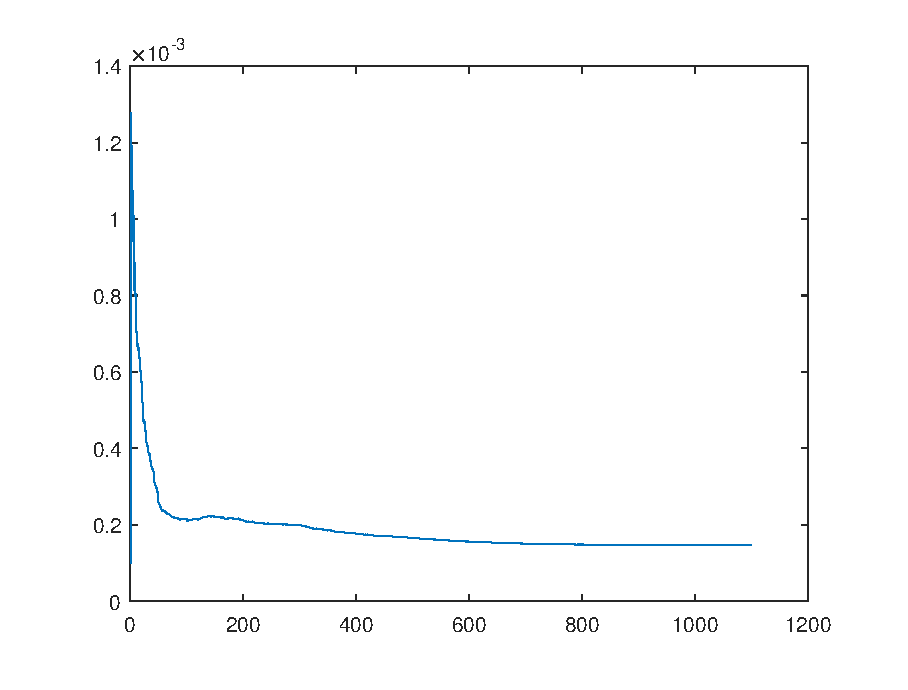
\includegraphics[width=\maxwidth{56.196688409433015em}]{figure_3.eps}
\end{center}
\begin{matlabcode}
figure;
plot(K,WRo);
\end{matlabcode}
\begin{center}
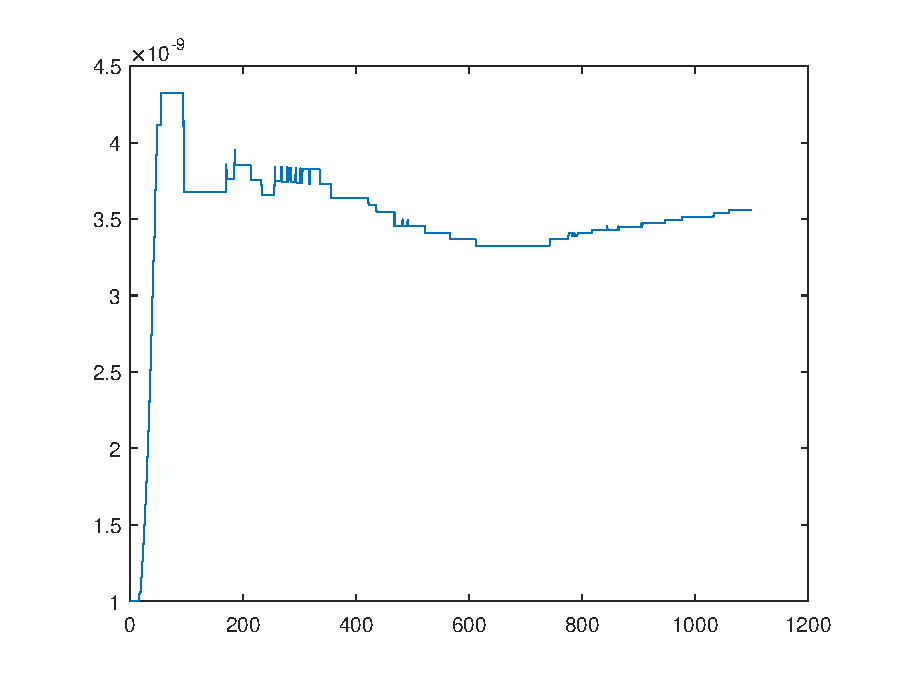
\includegraphics[width=\maxwidth{56.196688409433015em}]{figure_4.eps}
\end{center}
\begin{matlabcode}
figure;
plot(K,WTDiffusion);
\end{matlabcode}
\begin{center}
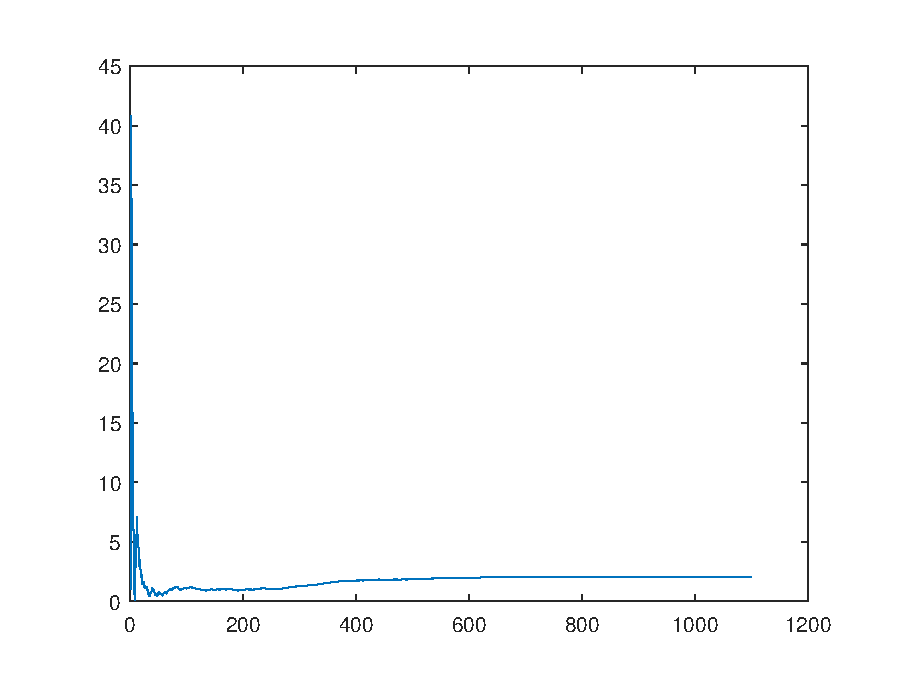
\includegraphics[width=\maxwidth{56.196688409433015em}]{figure_5.eps}
\end{center}
\begin{matlabcode}

% Test out for the last estimated value (should be most accurate)
wq = WQ(end);
QMobilePredicted(1) = QMobile(1);
for k=2:length(QMobile)
	QMobilePredicted(k) = QMobilePredicted(k-1) - wq*I(k-1)*Dt(k-1);
end
figure;
plot(K,QMobile,'b.',K,QMobilePredicted,'r.');
title('QMobile Observed and Predicted')
legend('Observed','Predicted');
\end{matlabcode}
\begin{center}
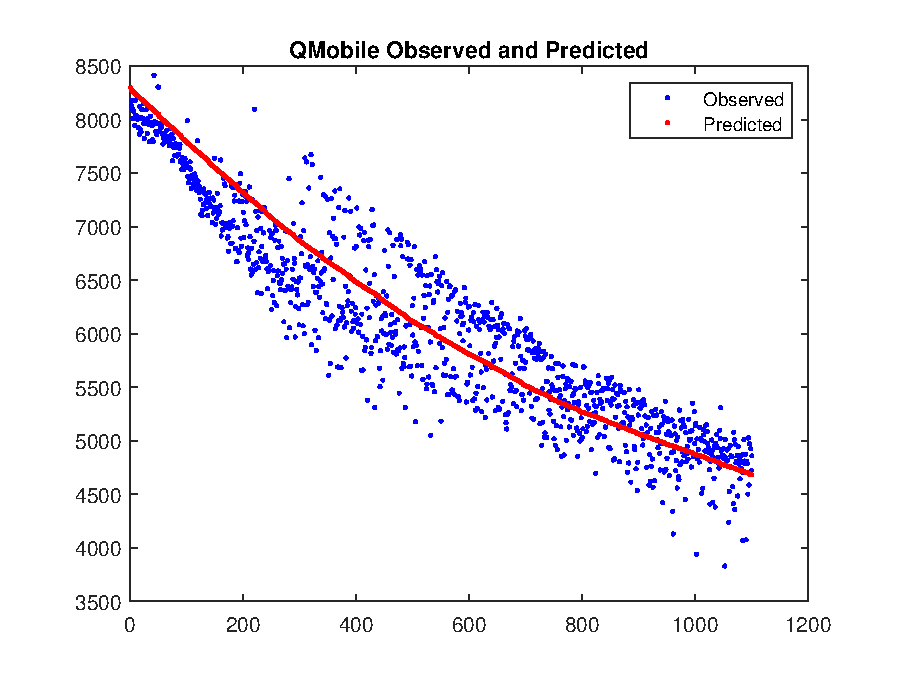
\includegraphics[width=\maxwidth{56.196688409433015em}]{figure_6.eps}
\end{center}
\begin{matlabcode}

% Test out for the last estimated value (should be most accurate)
wRo = WRo(end);
RoPredicted(1) = Ro(1);
for k=2:length(Ro)
	RoPredicted(k) = RoPredicted(k-1) + wR*I(k-1)*Dt(k-1);
end
figure;
plot(K,Ro,'b.',K,RoPredicted,'r.');
title('Ro Observed and Predicted')
legend('Observed','Predicted');
\end{matlabcode}
\begin{center}
\includegraphics[width=\maxwidth{56.196688409433015em}]{figure_7.eps}
\end{center}
\begin{matlabcode}

% Test out for the last estimated value (should be most accurate)
wTD = WTDiffusion(end);
TDiffusionPredicted(1) = TDiffusion(1);
for k=2:length(TDiffusion)
	TDiffusionPredicted(k) = TDiffusionPredicted(k-1) + wTD*I(k-1)*Dt(k-1);
end
figure;
plot(K,TDiffusion,'b.',K,TDiffusionPredicted,'r.');
title('TDiffusion Observed and Predicted')
legend('Observed','Predicted');
\end{matlabcode}
\begin{center}
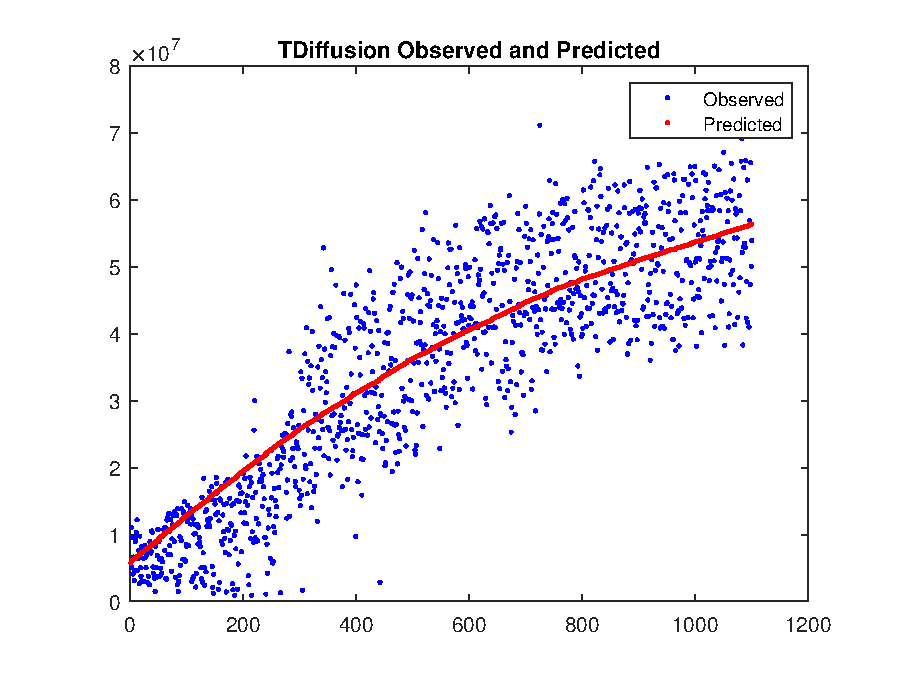
\includegraphics[width=\maxwidth{56.196688409433015em}]{figure_8.eps}
\end{center}
\begin{matlabcode}
addpath('C:\Users\mrmehta\Documents\GitHub\PrognosticsModelLibrary\MATLAB')
import Battery.*

% model.stateEqnHandle = @BatteryStateEqnCurrent;
% model.outputEqnHandle = @BatteryOutputEqnCurrent;
% model.inputEqnHandle = @BatteryInputEqnCurrent;
oneC = 2.021; %Default value
crate = 1;
loadval = oneC.*crate;
loads = [loadval;3600];
model = Battery.Create;
model.inputEqnHandle = @(P,t)Battery.InputEqn(P,t,loads);
% battery.inputEqnHandle = @(P,t)Battery.InputEqn(P,t);
[Ttosim,~,~,Z] = model.simulateToThreshold();
EOD_start = Ttosim(end);
plot(Ttosim, Z(2,:))
xlabel('Time [s]');
ylabel('Voltage [V]');
axis square
box on
ax = gca;
ax.Color = 'None';
\end{matlabcode}
\begin{center}
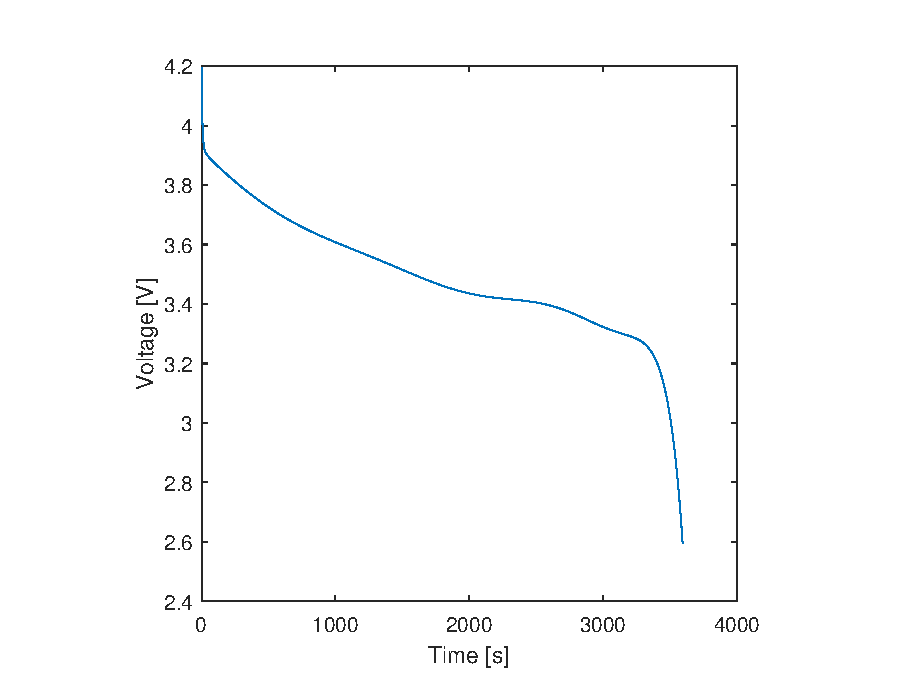
\includegraphics[width=\maxwidth{56.196688409433015em}]{figure_9.eps}
\end{center}
\begin{matlabcode}
fprintf('Discharge time: %gs',EOD_start);
\end{matlabcode}
\begin{matlaboutput}
Discharge time: 3594s
\end{matlaboutput}


\begin{matlabcode}
% Do EOL prediction - see when time for reference discharge would be at
% 50%. To do that, at each prediction time, we predict ahead what aging
% parameter values will be according to aging model and known I,Dt. At each
% future value (up to a point), run a reference discharge to see what
% discharge time will be.
% create battery model
import Battery.*
model = Battery.Create;
\end{matlabcode}
\begin{matlaboutput}
Unrecognized function or variable 'System'.

Error in BatteryEC8.createBattery (line 37)
S = System('Battery',P,@BatteryStateEqn,@BatteryInputEqn,@BatteryOutputEqn,...
\end{matlaboutput}
\begin{matlabcode}
% make sure model is using current as an input
% model.stateEqnHandle = @BatteryStateEqnCurrent;
% model.outputEqnHandle = @BatteryOutputEqnCurrent;
% model.inputEqnHandle = @BatteryInputEqnCurrent;
% for each "observation" point (every 100th actually)
for i=100:10:length(K) % start at 100 since no convergence before then
	% For this k, predict future values of Q,R,TD:
	QMobilePredicted(i) = QMobile(i); % use current value of qMobile
	wq = WQ(i);	% use current value of wq
	for k=i+1:length(QMobile)
		QMobilePredicted(k) = QMobilePredicted(k-1) - wq*I(k-1)*Dt(k-1);
	end
	RoPredicted(1) = Ro(i);
	wR = WRo(i);
	for k=i+1:length(Ro)
		RoPredicted(k) = RoPredicted(k-1) + wR*I(k-1)*Dt(k-1);
	end
	wTD = WTDiffusion(i);
	TDiffusionPredicted(i) = TDiffusion(i);
	for k=2:length(TDiffusion)
		TDiffusionPredicted(k) = TDiffusionPredicted(k-1) + wTD*I(k-1)*Dt(k-1);
	end
	% Now have predicted future values of aging parameters. For each of
	% these, compute what EOD time will be
	for k=i+mod(i+1,10):10:length(QMobile)
        curQmobile = QMobilePredicted(k);
		model.P = Battery.Parameters(curQmobile);
		model.P.Ro = RoPredicted(k);
		model.P.tDiffusion = TDiffusionPredicted(k);
		x0 = Battery.findX0(model,model.P.oneC,[4.2; 58.9]); % batterymodel, input current, [charge voltage, ambient temperature]
        
		model.P = BatteryEC8.BatteryParams(QMobilePredicted(k));
		model.P.Ro = RoPredicted(k);
		model.P.tDiffusion = TDiffusionPredicted(k);
		x0 = BatteryEC8.findX0(model,4.2,[4.2; 20]);
		tf = model.computeEOL(x0);
		if tf<3815
			EOL(i) = k;
			break;
		end
	end
end
\end{matlabcode}


\begin{matlabcode}
EOL = [];
EOD = [];
figure(10)
clf
xlabel('Time [s]');
ylabel('Voltage [V]');
axis square
box on
ax = gca;
ax.Color = 'None';
hold on
% plot(QMobilePredicted)
	for k=1:10:length(K)
        curQmobile = QMobilePredicted(k);
		model.P = Battery.Parameters(curQmobile);
% 		model.P.Ro = RoPredicted(k);
% 		model.P.tDiffusion = TDiffusionPredicted(k);
		x0 = Battery.findX0(model,model.P.oneC,[4.2; 58.9]); % batterymodel, input current, [charge voltage, ambient temperature]
        qpSMin  = x0(1);
        qpBMin  = x0(2);
        qnSMax  = x0(3);
        Vo      = x0(5);
        figure(10)
        plot(k, qpSMin,'k.',k, qpBMin,'b.',k, qnSMax,'r.',k, Vo,'g.')
        drawnow();

	end
\end{matlabcode}


\matlabheading{\textbf{Simulate ageing as mentioned in the "original code" with plots (no predictions)}}

\begin{matlabcode}
EOL = [];
EOD = [];
figure(10)
clf
xlabel('Time [s]');
ylabel('Voltage [V]');
axis square
box on
ax = gca;
ax.Color = 'None';
hold on
figure(11)
clf
xlabel('Time [s]');
ylabel('Voltage [V]');
axis square
box on
ax = gca;
ax.Color = 'None';
hold on
figure(12)
clf
xlabel('Time [s]');
ylabel('Voltage [V]');
axis square
box on
ax = gca;
ax.Color = 'None';
hold on
for i=100:10:length(K) % start at 100 since no convergence before then
	% For this k, predict future values of Q,R,TD:
	QMobilePredicted(i) = QMobile(i); % use current value of qMobile
	wq = WQ(i);	% use current value of wq
	for k=i+1:length(QMobile)
		QMobilePredicted(k) = QMobilePredicted(k-1) - wq*I(k-1)*Dt(k-1);
	end
	RoPredicted(1) = Ro(i);
	wR = WRo(i);
	for k=i+1:length(Ro)
		RoPredicted(k) = RoPredicted(k-1) + wR*I(k-1)*Dt(k-1);
	end
	wTD = WTDiffusion(i);
	TDiffusionPredicted(i) = TDiffusion(i);
	for k=2:length(TDiffusion)
		TDiffusionPredicted(k) = TDiffusionPredicted(k-1) + wTD*I(k-1)*Dt(k-1);
	end
	% Now have predicted future values of aging parameters. For each of
	% these, compute what EOD time will be
	for k=i+mod(i+1,10):10:length(QMobile)
        curQmobile = QMobilePredicted(k);
		model.P = Battery.Parameters(curQmobile);
		model.P.Ro = RoPredicted(k);
		model.P.tDiffusion = TDiffusionPredicted(k);
		x0 = Battery.findX0(model,model.P.oneC,[4.2; 58.9]); % batterymodel, input current, [charge voltage, ambient temperature]
        qpSMin  = x0(1);
        qpBMin  = x0(2);
        qnSMax  = x0(3);
        qnBMax  = x0(4);
        Vo      = x0(5);
        T       = x0(8);
        model.P.x0.qpS  = qpSMin;
        model.P.x0.qpB  = qpBMin;
        model.P.x0.qnS  = qnSMax;
        model.P.x0.qnB  = qnBMax;
        model.P.x0.Vo   = Vo;
        model.P.x0.Tb   = T;
		[Ttosim,~,~,Z]  = model.simulateToThreshold();
        figure(12)
        if ~any(any(imag(Z)))
            hold on;plot(k,Z(2,1),'k.');hold off;drawnow();
        end
        tf = Ttosim(end);
%         fprintf('Discharge time: %gs\n',tf);
		if tf<EOD_start && tf>(EOD_start/2)
%             fprintf('Discharge time: %gs\n',tf);
            figure(10)
            plot(Ttosim, Z(2,:))
            drawnow();
            figure(11)
            plot(Ttosim, Z(1,:))
            drawnow();            
			EOL(length(EOL)+1) = k;
            EOD(length(EOD)+1) = tf;
			break;
        else
            continue;
		end
	end

    end
drawnow();
hold off
\end{matlabcode}


\matlabheading{Simulate ageing as mentioned in the "original code" (w predictions and no plots)}

\begin{matlabcode}
EOL = nan.*ones(length(QMobile),1);
EOD = nan.*ones(length(QMobile),1);
for i=100:10:length(K) % start at 100 since no convergence before then
	% For this k, predict future values of Q,R,TD:
	QMobilePredicted(i) = QMobile(i); % use current value of qMobile
	wq = WQ(i);	% use current value of wq
	for k=i+1:length(QMobile)
		QMobilePredicted(k) = QMobilePredicted(k-1) - wq*I(k-1)*Dt(k-1);
	end
	RoPredicted(1) = Ro(i);
	wR = WRo(i);
	for k=i+1:length(Ro)
		RoPredicted(k) = RoPredicted(k-1) + wR*I(k-1)*Dt(k-1);
	end
	wTD = WTDiffusion(i);
	TDiffusionPredicted(i) = TDiffusion(i);
	for k=i+1:length(TDiffusion)
		TDiffusionPredicted(k) = TDiffusionPredicted(k-1) + wTD*I(k-1)*Dt(k-1);
	end
	% Now have predicted future values of aging parameters. For each of
	% these, compute what EOD time will be
	for k=i+mod(i+1,10):10:length(QMobile)
        curQmobile = QMobilePredicted(k);
		model.P = Battery.Parameters(curQmobile);
		model.P.Ro = RoPredicted(k);
		model.P.tDiffusion = TDiffusionPredicted(k);
		x0 = Battery.findX0(model,model.P.oneC,[4.2; 58.9]); % batterymodel, input current, [charge voltage, ambient temperature]
        qpSMin  = x0(1);
        qpBMin  = x0(2);
        qnSMax  = x0(3);
        qnBMax  = x0(4);
        Vo      = x0(5);
        T       = x0(8);
        model.P.x0.qpS  = qpSMin;
        model.P.x0.qpB  = qpBMin;
        model.P.x0.qnS  = qnSMax;
        model.P.x0.qnB  = qnBMax;
        model.P.x0.Vo   = Vo;
        model.P.x0.Tb   = T;
		[Ttosim,~,~,~]  = model.simulateToThreshold();
        tf = Ttosim(end);
        EOD(k) = tf;
% Assuming the Crate is 1C, the total discharge time is 1hr. The EOL is
% when the battery reaches 80% SOH (a commonly used criteria)
        
		if tf<3600*0.8 % 1hr at 80% loss
			EOL(i) = k;
			break;
		end
	end
end
\end{matlabcode}


\matlabheadingtwo{\textbf{Simulate ageing as mentioned in the "original code" (wo predictions and no plots)}}

\begin{matlabcode}
EOL = nan.*ones(length(QMobile),1);
EOD = nan.*ones(length(QMobile),1);
for i=100:10:length(K) % start at 100 since no convergence before then
	for k=i+mod(i+1,10):10:length(QMobile)
        curQmobile = QMobilePredicted(k);
		model.P = Battery.Parameters(curQmobile);
		model.P.Ro = RoPredicted(k);
		model.P.tDiffusion = TDiffusionPredicted(k);
		x0 = Battery.findX0(model,model.P.oneC,[4.2; 58.9]); % batterymodel, input current, [charge voltage, ambient temperature]
        qpSMin  = x0(1);
        qpBMin  = x0(2);
        qnSMax  = x0(3);
        qnBMax  = x0(4);
        Vo      = x0(5);
        T       = x0(8);
        model.P.x0.qpS  = qpSMin;
        model.P.x0.qpB  = qpBMin;
        model.P.x0.qnS  = qnSMax;
        model.P.x0.qnB  = qnBMax;
        model.P.x0.Vo   = Vo;
        model.P.x0.Tb   = T;
		[Ttosim,~,~,~]  = model.simulateToThreshold();
        tf = Ttosim(end);
        EOD(k) = tf;
% Assuming the Crate is 1C, the total discharge time is 1hr. The EOL is
% when the battery reaches 80% SOH (a commonly used criteria)
        tEOL = 3600*0.8;
		if tf<tEOL % 1hr at 80% loss
			EOL(i) = k;
			break;
		end
    end
    if i==k-1
        break;
    end
end
\end{matlabcode}


\matlabheading{Simulate cycles without predicting the degradation values}

\begin{matlabcode}
EOL = [];
EOD = [];
figure(11)
clf
xlabel('Time [s]');
ylabel('Temperature [\circC]');
axis square
box on
ax = gca;
ax.Color = 'None';
hold on
figure(10)
clf
xlabel('Time [s]');
ylabel('Voltage [V]');
axis square
box on
ax = gca;
ax.Color = 'None';
hold on
tlast = 3700;
oneC = 2.021; %Default value
crate = 1;
loadval = oneC.*crate;
loads = [loadval;3600];
model = Battery.Create;
model.inputEqnHandle = @(P,t)Battery.InputEqn(P,t,loads);
[Ttosim,~,~,Z] = model.simulateToThreshold();
EOD_start = Ttosim(end);
figure(10)
plot(Ttosim, Z(2,:),'DisplayName','Cycle 1')
drawnow();
figure(11)
plot(Ttosim, Z(1,:),'DisplayName','Cycle 1')
drawnow();         
forloopvals = 100:100:length(K);
nforloop = length(forloopvals);
initvolt = ones(length(nforloop),1);
qpSMinvals = ones(length(nforloop),1);
qpBMinvals = ones(length(nforloop),1);
qnSMaxvals = ones(length(nforloop),1);
qnBMaxvals = ones(length(nforloop),1);
Vovals = ones(length(nforloop),1);
Tmax = ones(length(nforloop),1);
Vepvals = ones(length(nforloop),1);
Venvals = ones(length(nforloop),1);
E0vals = ones(length(nforloop),1);
for i=1:nforloop
    k = forloopvals(i);
    curQmobile = QMobilePredicted(k);
	model.P = Battery.Parameters(curQmobile);
	model.P.Ro = RoPredicted(k);
	model.P.tDiffusion = TDiffusionPredicted(k);
	x0 = BatteryEC8.findX0(model,model.P.oneC,[4.2; 58.9]); % batterymodel, input current, [charge voltage, ambient temperature]
    qpSMin  = x0.qpS0;
    qpBMin  = x0.qpB0;
    qnSMax  = x0.qnS0;
    qnBMax  = x0.qnB0;
    Vo      = x0.Vo;
    T       = x0.T;
    Vep = x0.Vep0;
    Ven = x0.Ven0;
    E0 = x0.E0; 
    qpSMinvals(i) = qpSMin;
    qpBMinvals(i) = qpBMin;
    qnSMaxvals(i) = qnSMax;
    qnBMaxvals(i) = qnBMax;
    Vovals(i) = Vo;
    Vepvals(i) = Vep;
    Venvals(i) = Ven;
    E0vals(i) = E0;
    model.P.x0.qpS  = qpSMin;
    model.P.x0.qpB  = qpBMin;
    model.P.x0.qnS  = qnSMax;
    model.P.x0.qnB  = qnBMax;
    model.P.x0.Vo   = Vo;
    model.P.x0.Tb   = T;
	[Ttosim,~,~,Z]  = model.simulateToThreshold();
    Tmax(i) = Z(1,end);
    initvolt(i) = Z(2,1);
    tf = Ttosim(end);
    if tf<EOD_start && tf>(EOD_start/2)
        figure(10)
        plot(Ttosim, Z(2,:),'DisplayName',['Cycle ' num2str(k)])
        drawnow();
        figure(11)
        plot(Ttosim, Z(1,:),'DisplayName',['Cycle ' num2str(k)])
        drawnow();            
		EOL(i) = k;
        EOD(i) = tf;
    else
        continue;
    end
end
figure(10)
legend("Location","best")
\end{matlabcode}
\begin{center}
\includegraphics[width=\maxwidth{56.196688409433015em}]{figure_10.png}
\end{center}
\begin{matlabcode}
figure(11)
legend("Location","best")
\end{matlabcode}
\begin{center}
\includegraphics[width=\maxwidth{56.196688409433015em}]{figure_11.png}
\end{center}


\begin{matlabcode}
figure
yyaxis left
plot(forloopvals,initvolt,'k-',"LineWidth",1);
% title('Initial Voltage')
axis square
xlabel('Cycles')
ylabel('OCV [V]')
% figure
ax = gca;
ax.YColor='k';
% Color = 'k';
yyaxis right
plot(forloopvals,Tmax,'b-',"LineWidth",1);
% title('Maximum Temperature')
ax = gca;
ax.YColor='b';
axis square
ylabel('Temperature [\circC]')
figure
plot(forloopvals,Vepvals,'k-',"LineWidth",1,'DisplayName','Cathode');
hold on;plot(forloopvals,Venvals,'b-',"LineWidth",1,'DisplayName','Anode');hold off;
axis square
xlabel('Cycles')
ylabel('Decoupled OCV [V]')
figure(1)
subplot(2,2,1)
plot(forloopvals,qpSMinvals,'k-');
title('qpSMin')
axis square
xlabel('Cycles')
subplot(2,2,2)
plot(forloopvals,qpBMinvals,'b-');
title('qpBMin')
axis square
xlabel('Cycles')
subplot(2,2,3)
plot(forloopvals,qnSMaxvals,'g-');
title('qnSMax')
axis square
xlabel('Cycles')
subplot(2,2,4)
plot(forloopvals,qnBMaxvals,'r-');
title('qnBMax')
axis square
xlabel('Cycles')        
\end{matlabcode}


\begin{matlabcode}
figure
plot(110:10:length(K),EOL,'o')
axis square
figure
plot(110:10:length(K),EOD,'bo','MarkerFaceColor','b','MarkerSize',4)
axis square
figure
plot(110:10:length(K),oneC.*EOD./3600,'bo','MarkerFaceColor','b','MarkerSize',4)
hold on
plot([110,length(K)],[1.6168,1.6168],'r-','LineWidth',1.5)
hold off
axis square
\end{matlabcode}


\begin{matlabcode}
[Ttosim,~,~,Z] = model.simulateToThreshold();
EOD_current = Ttosim(end);
fprintf('Discharge time: %gs',EOD_current);
fprintf('SOH: %0.2f%%',(EOD_current/EOD_start)*100);
\end{matlabcode}


\begin{matlabcode}
function e = optQMobile(wq,QMobile,I,Dt,kEnd)
    QMobilePredicted(1) = QMobile(1);
    for k=2:kEnd
    	QMobilePredicted(k) = QMobilePredicted(k-1) - wq*I(k-1)*Dt(k-1);
    end
    e = sum((QMobilePredicted-QMobile(1:kEnd)).^2);
end
% Here is the optimization function for Ro
function e = optRo(wRo,Ro,I,Dt,kEnd)
    RoPredicted(1) = Ro(1);
    for k=2:kEnd
    	RoPredicted(k) = RoPredicted(k-1) + wRo*I(k-1)*Dt(k-1);
    end
    e = sum((RoPredicted-Ro(1:kEnd)).^2);
end
% Here is the optimization function for tDiffusion
function e = optTDiffusion(wTD,TDiffusion,I,Dt,kEnd)
    TDiffusionPredicted(1) = TDiffusion(1);
    for k=2:kEnd
    	TDiffusionPredicted(k) = TDiffusionPredicted(k-1) + wTD*I(k-1)*Dt(k-1);
    end
    e = sum((TDiffusionPredicted-TDiffusion(1:kEnd)).^2);
end
\end{matlabcode}

\end{document}
